\chapter{Vyhledávání relevantních obrázků}
\label{chap:teorie}

% \section{Teoretické cíle}

% V teoretické části je hlavním cílem práce nalézt nejvhodnější metodu extrakce klíčových slov textu. Tato klíčová slova pak budou použita při vyhledávání ilustračních obráyků v databázi Profimedie. Celá práce, pokud nebude uvedeno jinak, označuje za slova stemy vstupních slov. Jako stemmer se využívá ??? stemmer.

% Vstupní text tedy nejprve rozdělíme na slova. Čísla a interpunkce nás v této úloze nezajímají, jelikož se v datech nenachází. Ze slov pak získáme stemy. Vstupem algoritmu pro nalezení klíčových slov tedy bude množina vhodných stemů. Ke každému stemu si ještě uložíme jednu jeho nestemovou variantu, kterpu pak můžeme zobrazit uživateli.

% Nyní můžeme použít některý z algoritmů na extrakci klíčových slov uvedených v další kapitole.

\begin{figure}[h]
  \centering
  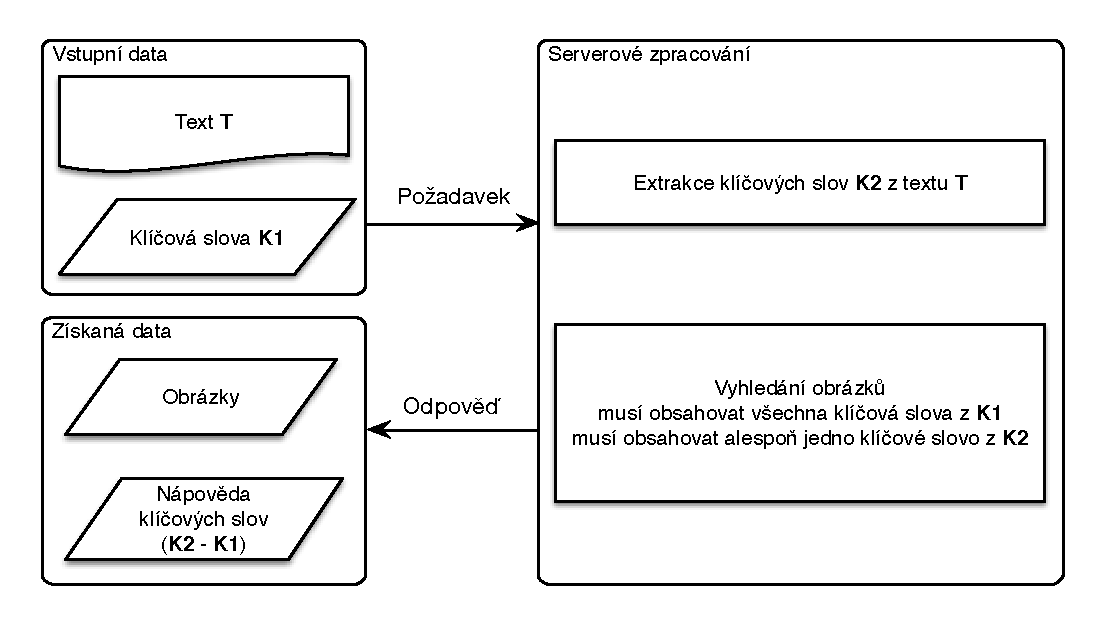
\includegraphics[width=150mm]{dataflow.eps}
  \caption{Základní tok dat mezi klientem a serverem.}
  \label{fig:dataflow}
\end{figure}


Aplikace poskytuje uživateli dvě možnosti vyhledávání. Základním uživatelským scénářem je vložit do rozhraní text. Aplikace by v takovém případě měla poskytnout relevantní obrázky k danému textu. V dalším uživatelském scénáři je přímý požadavek na klíčová slova obrázku. Uživatel by měl mít možnost zadat přímo klíčová slova, které metadata k nalezeným obrázkům musí obsahovat. Oba scénáře by mělo navíc být možné propojit pomocí nápovědy klíčových slov -- uživatel zadá do rozhraní text, dostane výsledné obrázky a nápovědu klíčových slov, kterými může množinu nalezených obrázků více omezit. Celý proces hledání vhodných obrázků popisuje diagram \ref{fig:dataflow}.

\section{Extrakce klíčových slov}

Extrakce klíčových slov je velmi důležitou složkou celého vyhledávání. Článek \cite{lott} shrnuje základní techniky extrakce klíčových slov z textu. Algoritmy na extrakci klíčových slov lze v zásadě rozdělit do dvou kategorií - \uv{s korpusem} a \uv{bez korpusu}. Metody pracující bez korpusu jsou zajímavé a mohou dosahovat podobných výsledků jako metody s korpusem. My však máme k dispozici dataset Profimedie, takže o metody pracující bez korpusu se tato práce dále nezajímá. 

\section{TF-IDF}

TF-IDF je jeden ze základních vyhledávacích algoritmů. Algoritmus využívá korpusu dokumentů $D$ a dvou složek $TF$ a $IDF$, lze ho vyjádřit jako rovnost

\begin{equation}
  TFIDF(t,d,n,N)= TF(t,d)\times IDF(n,N).
\end{equation}

Složka $TF$ znamená $TERM\ FREQUENCY$ a pokud $t$ je slovo a $d \in D$ je dokument, je $TF$

\begin{equation}
 TF(t,d) = \sum_{slovo\,\in\,d} \begin{array}{l l} 1 & \mathrm{pokud}\ slovo = t \\
  0 & \mathrm{jinak} \end{array}.
\end{equation}

Jedná se tedy o frekvenci slova v dokumentu.

Složka $IDF$, tedy $INVERSE\ DOCUMENT\ FREQUENCY$ vyjadřuje, jak moc daný termín popisuje dokument. Pokud je $N$ počet všech dokumentů v $D$, tedy $N = |D|$ a $n$ je počet dokumentů, ve kterých se vyskytuje slovo $t$, je $IDF$ tohoto slova

\begin{equation}
IDF(n,N) = \log \left(\frac{N}{n}\right).
\end{equation}

Čím je tedy slovo v korpusu častější, tím více se s logaritmem snižuje jeho informační hodnota. Slova, která jsou velmi běžná, většinou klíčovými slovy nejsou.

Výsledný vzorec pak jde shrnout jako

\begin{equation}
TFIDF(t,d,n,N)= \left(\sum_{slovo\,\in\,d} \begin{array}{l l} 1 & \mathrm{pokud}\ slovo = t \\
  0 & \mathrm{jinak} \end{array}\right)
  \times
  \log \left(\frac{N - n}{n}\right).
\end{equation}

\section{TF-IDF pro extrakci klíčových slov}
\label{sec:keywords_extraction}

Algortimus TF-IDF můžeme použít pro extrakci klíčových slov z textu. Všechna znaky vstupního textu převedeme na malá písmena a text rozdělíme na slova. Odstraníme slova ze stop-slovníku, který obsahuje nejběžnější slova pro každý z podporovaných jazyků\footnote{Seznam slov ve stopslovnících je převzat z knihovny Lucene.}. Dále nás nezajímá diakritika a různé speciální znaky, které může text obsahovat.  Slova převedeme na stemy. O převodu slov na stemy se podrobněji píše v Kapitole \ref{chap:stemmer}.

Algoritmus TF-IDF pak použijeme na každé slovo vstupního textu a získáme tak skóre jeho významnosti v textu. Slova s nejvyšším skóre pak označíme za klíčová. Algoritmus musíme upravit pro naše účely. Zaprvé nás zajímají pouze taková slova, která existují v datasetu Profimedie. Slova, která se v korpusu nenachází, dostanou skóre $0$. Část TF v algoritmu znamená četnost slova v textu.

Složitější je situace s $IDF$. Nabízí se použít frekvenci slov z datasetu Profimedie. Ukázalo se, že klíčová slova obrázků z datasetu nejsou pro tento účel vhodná. Klíčová slova totiž obsahují mnoho názvů a obecně méně běžných slov. Naopak obsahují velmi málo běžných slov. To pak způsobuje, že algoritmus na tomto datasetu přiřazuje vysoké skóre běžným slovům. Tato slova ale typicky nejsou vhodnými klíčovými slovy daného textu. Je tedy potřeba použít pro vzorec $DF$ jiný korpus. V naší aplikaci jsme použili korpus Wikipedie, jejíž data jsou volně dostupná pro mnoho jazyků pod otevřenou licencí.

Pokud je $w$ slovo vstupního textu, $Freq(w)$ je četnost slova ve vstupním textu a $Wiki(w)$ je četnost slova v korpusu Wikipedie, můžeme každému slovu vstupního slova přířadit $Score$:


\begin{equation}
  Score(w) = \left\{
  \begin{array}{l l} Freq(w) \times (\frac{C}{Wiki(w)}) & w\ \mathrm{je\ v\ datasetu\ Profimedie} \\
  0 & w\ \mathrm{není\ v\ datasetu\ Profimedie}
  \end{array}
  \right.
\end{equation}

$C$ je experimentálně zjištěná konstanta. V našem případě je její hodnota $10\ 000\ 000$.

Nyní tedy máme skóre udávající význam slova pro každé slovo vstupního textu. Slova s nejvyšším skóre vrátíme uživateli jako nápovědu pro explicitní požadavek obrázků s klíčovými slovy.


\section{Vyhledávání obrázků}

Samotné vyhledávání obrázků má dva druhy vstupních dat. Prvním typem je text článku, který uživatel vloží do uživatelského rozhraní. Máme tedy k dispozici řetězec s textem článku. Dále může uživatel zadat explicitní klíčová slova, které má hledaný obrázek obsahovat. Tato vstupní data získáváme jako pole řetězců. Úkolem algoritmu na vyhledávání obrázků je vrátit uživateli všechny relevantní obrázky v pořadí podle relevance.

Text si nejprve zpracujeme pomocí algoritmu uvedeném v sekci \ref{sec:keywords_extraction}. Získáme skóre významnosti pro všechna slova ve vstupním textu. Pro vyhledávání použijeme pouze několik slov s nejvyšším skóre.

Nyní můžeme jako množinu relevantních obrázků označit obrázky, které ve svých klíčových slovech mají všechna uživatelem zadaná explicitní klíčová slova a alespoň jedno klíčové slovo získané extrakcí klíčových slov z textu.

Množina relevantních obrázků může být velká a obsahovat obrázky, které jsou relevantní jen velmi málo. Je proto důležité množinu relevantních obrázků správně seřadit. Máme množinu $K_{text}$ klíčových slov získaných z textu. Každé $w \in K_{text}$ má skóre $Score(w)$. Relevantní obrázek má množinu klíčových slov $K_{img}$. Relevanci obrázku vůči uživatelskému dotazu můžeme ohodnotit funkcí $Rank$:

\begin{equation}
Rank(K_{text}, K_{img}) = \sum_{w \in K_{text}}{
  \left\{
  \begin{array}{l l} Score(w) \times \frac{1}{|K_{img}|} & w\ \in K_{img} \\
  0 & w \notin K_{img}
  \end{array}
  \right.
}
\end{equation}

Vzorec bere v úvahu počet klíčových slov, které obrázek obsahuje. Snižuje relevanci obrázků, které obsahují mnoho klíčových slov a zvýhodňuje tím ve vyhledávání obrázky, které mají menší počet přesnějších klíčových slov.




